\documentclass[tikz, border=10pt]{standalone}
\usepackage{iftex}
\ifluatex
  \usepackage{fontspec}
  \usepackage{unicode-math}
  \setmainfont{Fira Sans}
  \setmonofont{Fira Mono}
  \setmathfont{Fira Math}
  \setmathfont{STIX Two Math}[range={"29F5,"2216}]
\else
  \usepackage[T1]{fontenc}
\fi

\usepackage{amsmath}
\usepackage{tikz}
\usetikzlibrary{arrows.meta}
\tikzset{every node/.style={font=\Large}}

% Theme toggle: \darkbgfalse for light background preview.
\newif\ifdarkbg
\darkbgfalse
\ifdarkbg
  \colorlet{axiscol}{white}
  \colorlet{gridcol}{white!30!black}
  \colorlet{ticklabelcol}{white}
  \colorlet{funcol}{yellow!85!white}
  \colorlet{auxcol}{white!50!black}
\else
  \colorlet{axiscol}{black}
  \colorlet{gridcol}{black!25!white}
  \colorlet{ticklabelcol}{black}
  \colorlet{funcol}{blue!70!black}
  \colorlet{auxcol}{black!40!white}
\fi

% x: -4 to 5   (9 units)   xscale=0.8  → ~7.2 cm wide
% y: -6 to  5  (11 units)  yscale=0.65 → ~7.2 cm tall  (square)
% Vertical asymptote at x = -3.  Domain: x > -3.
% f(5) = -2·log₂(8) = -6  → curve exits exactly at the bottom border.
% Integer points: (-2,0)  (-1,-2)  (1,-4)  (5,-6)
\begin{document}
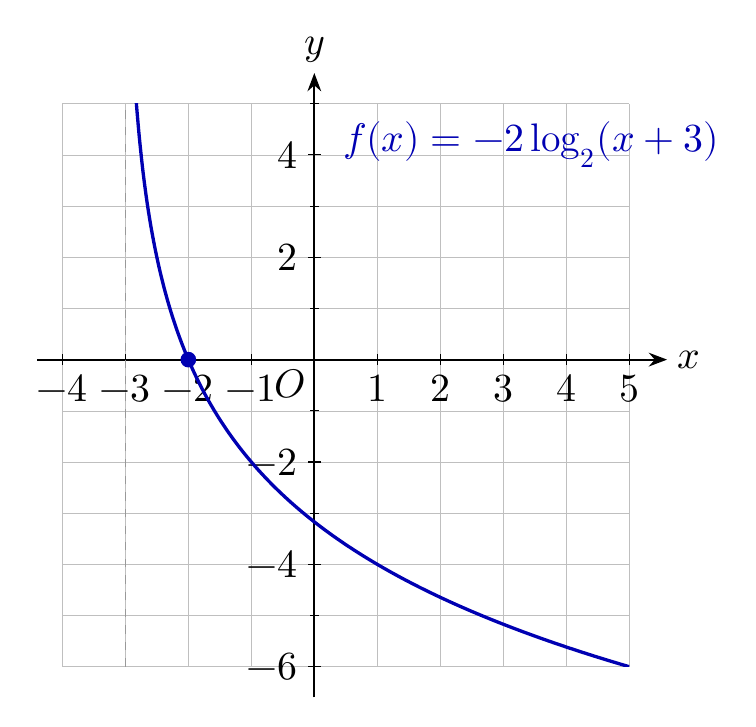
\begin{tikzpicture}[xscale=0.8, yscale=0.65, >=Stealth]

  % Cartesian grid.
  \draw[step=1, very thin, gridcol] (-4,-6) grid (5,5);

  % Axes.
  \draw[->, thick, axiscol] (-4.4,0) -- (5.6,0)
    node[right, text=axiscol] {$x$};
  \draw[->, thick, axiscol] (0,-6.6) -- (0,5.6)
    node[above, text=axiscol] {$y$};

  % Tick marks — x axis.
  \foreach \x in {-4,-3,-2,-1,1,2,3,4,5} {
    \draw[axiscol] (\x, 3pt) -- (\x, -3pt)
      node[below, text=ticklabelcol] {$\x$};
  }

  % Tick marks — y axis (labelled every 2, minor every 1).
  \foreach \y in {-6,-4,-2,2,4} {
    \draw[axiscol] (3pt,\y) -- (-3pt,\y)
      node[left, text=ticklabelcol] {$\y$};
  }
  \foreach \y in {-5,-3,-1,1,3,5} {
    \draw[axiscol] (2pt,\y) -- (-2pt,\y);
  }

  % Origin label.
  \node[below left, text=axiscol] at (0,0) {$O$};

  % Vertical asymptote x = -3 (dashed).
  \draw[dashed, auxcol] (-3,-6) -- (-3,5);

  % Function curve: f(x) = -2·log₂(x+3) = -2·ln(x+3)/ln(2)
  % Clipped to window; domain starts just right of the asymptote.
  \begin{scope}
    \clip (-4,-6) rectangle (5,5);
    \draw[domain=-2.993:5, smooth, very thick, funcol, samples=120]
      plot (\x, {-2*ln(\x+3)/ln(2)});
  \end{scope}

  % Function label — upper area, above the curve.
  \node[right, text=funcol] at (0.3,4.2) {$f(x)=-2\log_2(x+3)$};

  % Key points.
  \node[circle, fill=funcol, inner sep=2pt] at (-2,0)  {};  % x-intercept
  % \node[circle, fill=funcol, inner sep=2pt] at (-1,-2) {};
  % \node[circle, fill=funcol, inner sep=2pt] at (1,-4)  {};

\end{tikzpicture}
\end{document}
